%%% LaTeX Template: Article/Thesis/etc. with colored headings and special fonts
%%%
%%% Source: http://www.howtotex.com/
% vim: set spell spelllang=es syntax=tex :

\documentclass[12pt]{article}
\usepackage{styles/apuntes-estilo}
\usepackage{fancyhdr,lastpage}
\usepackage{hyperref}
\usepackage[inline]{enumitem}
\usepackage{xurl}
\usepackage{nameref}

\def\maketitle{

\makeatletter{
    \color{blue} \centering \huge \sc
    \textbf{
        Trabajo práctico N° 3\\
        \large \vspace*{-8pt} \color{black}
        Representación digital de datos: Texto y Multimedia
        \vspace*{8pt}
    }\\
    \small Fecha de finalización: 28 de abril
    \par
}

\makeatother

\makeatletter
% vim: set spell spelllang=es syntax=tex :
 {\centering \small 
    Introducción a la computación\\
    Departamento de Ingeniería de Computadoras \\
    Facultad de Informática - Universidad Nacional del Comahue \\
    \vspace{20pt} }
\makeatother

\vspace{-2.5cm}
\mbox{\hspace{-1cm}\includegraphics[width=3cm,height=3cm]{logos/uncoma.pdf}\hspace{12cm}
    
\includegraphics[width=3cm,height=3cm]{logos/fai.pdf}}



}

% Custom headers and footers
\fancyhf{} % clear all header and footer fields
\fancypagestyle{plain}{\fancyhf{}}
\pagestyle{fancy}
\lhead{\footnotesize TP N° 3 - Representación digital de datos: Texto y
Multimedia}
\rhead{\footnotesize \thepage\ }

\def\ti#1#2{\texttt{#1} & #2 \\ }

\begin{document}

\thispagestyle{empty}
\maketitle
\setlength{\parindent}{1pt}

\textbf{Objetivo:} comprender la representación binaria de texto, imagenes y
otros datos más complejos.

\textbf{Recursos bibliográfico:}

\vspace{-2\topsep}
\begin{itemize}

    \itemsep2pt \parskip0pt \parsep0pt
    \item Wikipedia: \emph{Run-length encoding}:
        \url{https://en.wikipedia.org/wiki/Run-length_encoding}
    
    \item Wikipedia: \emph{ASCII}:
        \url{http://es.wikipedia.org/wiki/ASCII}

\end{itemize}

\textbf{Recursos:}

\vspace{-2\topsep}
\begin{itemize}

    \itemsep2pt \parskip0pt \parsep0pt

    \item Tabla de caracteres ASCII Extendida:
        \url{http://www.programasprogramacion.com/caracteres.php}

    \item Tabla de caracteres \emph{UTF-8}:
        \url{http://www.fileformat.info/info/charset/UTF-8/list.htm}

\end{itemize}

\textbf{Tabla \emph{ASCII}:}
\begin{verbatim}
Dec Hex    Dec Hex    Dec Hex  Dec Hex  Dec Hex  Dec Hex   Dec Hex   Dec Hex  
  0 00 NUL  16 10 DLE  32 20    48 30 0  64 40 @  80 50 P   96 60 `  112 70 p
  1 01 SOH  17 11 DC1  33 21 !  49 31 1  65 41 A  81 51 Q   97 61 a  113 71 q
  2 02 STX  18 12 DC2  34 22 "  50 32 2  66 42 B  82 52 R   98 62 b  114 72 r
  3 03 ETX  19 13 DC3  35 23 #  51 33 3  67 43 C  83 53 S   99 63 c  115 73 s
  4 04 EOT  20 14 DC4  36 24 $  52 34 4  68 44 D  84 54 T  100 64 d  116 74 t
  5 05 ENQ  21 15 NAK  37 25 %  53 35 5  69 45 E  85 55 U  101 65 e  117 75 u
  6 06 ACK  22 16 SYN  38 26 &  54 36 6  70 46 F  86 56 V  102 66 f  118 76 v
  7 07 BEL  23 17 ETB  39 27 '  55 37 7  71 47 G  87 57 W  103 67 g  119 77 w
  8 08 BS   24 18 CAN  40 28 (  56 38 8  72 48 H  88 58 X  104 68 h  120 78 x
  9 09 HT   25 19 EM   41 29 )  57 39 9  73 49 I  89 59 Y  105 69 i  121 79 y
 10 0A LF   26 1A SUB  42 2A *  58 3A :  74 4A J  90 5A Z  106 6A j  122 7A z
 11 0B VT   27 1B ESC  43 2B +  59 3B ;  75 4B K  91 5B [  107 6B k  123 7B {
 12 0C FF   28 1C FS   44 2C ,  60 3C <  76 4C L  92 5C \  108 6C l  124 7C |
 13 0D CR   29 1D GS   45 2D -  61 3D =  77 4D M  93 5D ]  109 6D m  125 7D }
 14 0E SO   30 1E RS   46 2E .  62 3E >  78 4E N  94 5E ^  110 6E n  126 7E ~
 15 0F SI   31 1F US   47 2F /  63 3F ?  79 4F O  95 5F _  111 6F o  127 7F DEL
\end{verbatim}

\textbf{Lectura obligatoria:}

\vspace{-2\topsep}
\begin{itemize}

    \itemsep2pt \parskip0pt \parsep0pt

    \item Apuntes de cátedra. Capitulo 4:Representación digital de datos:
        Texto y Multimedia. Disponible en \textit{PEDCO}:
        \url{https://pedco.uncoma.edu.ar/mod/url/view.php?id=203642}

\end{itemize}

\textbf{Nota}: El prefijo ``\textbf{0x}'' indica que un número está en
hexadecimal.

\section{Codificación de texto}

\begin{enumerate}

    \item Decodifique los siguientes mensajes codificados en \emph{UTF-8} y
        representados en hexadecimal.

        \begin{enumerate}

            \item \textbf{41 79 75 64 61}

            \item \textbf{45 6C 20 C3 B1 61 6E 64 C3 BA 20 62 61 6A C3 B3 20
                65 6C 20 C3 A1 72 62 6F 6C}

            \item \textbf{48 6F 6C 61 20 6D 75 6E 64 6F}

            \item Para cada uno de los mensajes anteriores, responda: ¿cuántos
                caracteres posee? ¿cuántos bytes ocupa?

        \end{enumerate}

    \item Codifique su apellido y legajo en \emph{ASCII}, respetando
        el siguiente formato: ``\textit{Apellido} (\textit{legajo})''.
        Remplace aquellos caracteres que no puedan ser representados por el
        símbolo ``\textbf{?}''.

\end{enumerate}

\section{Representación de imágenes}
\label{sec_imagenes}

Los archivos de imagen utilizados en los ejercicios respetan el siguiente
formato:

\begin{tabular}[t]{|c|c|c||c|}

    \hline

    Ancho&Alto& Bits por pixel & Datos de la imagen\\

    \emph{1 byte}& \emph{1 byte}& \emph{1 byte}&\\

    \hline

\end{tabular}

\emph{Por simplicidad, el formato no incluye la paleta de colores}

\textbf{Ejemplo} dado un archivo de imagen cuyo contenido expresado en hexadecimal es:
        ``\textbf{04 06 01 69 12 4F}'' y cuyo formato es el descripto en la
        teoría, para poder obtener la imagen se deben seguir los siguientes
        pasos:

\begin{enumerate}
    \itemsep2pt \parskip0pt \parsep0pt

    \item Extraer los datos de la cabecera de la imagen: \emph{ancho},
        \emph{alto}, y \emph{bits por pixel}:

        \begin{itemize}
            \itemsep2pt \parskip0pt \parsep0pt

            \item \textbf{Ancho}: 4 pixeles.
            \item \textbf{Alto}: 6 pixeles.
            \item \textbf{Bits por pixel}: 1 bit por pixel.

        \end{itemize}

    \item Representar en binario los datos de la imagen:

        $0100\,1001\,0001\,0010\,0100\,1111$

    \item Crear una cuadricula de \emph{ancho}$x$\emph{alto} pixeles.

    \item Tomando de a ``\emph{bits por pixel}'' de los datos de la imagen,
        rellenar la cuadricula, comenzando desde la esquina superior
        izquierda, completando las filas:

        \begin{tabular}[t]{c|c}

            \emph{Datos de la imagen} & \emph{Imagen}\\

            \begin{tabular}{c|c}
                \emph{Hex.} & \emph{Binario}\\
                \hline
                6&0110\\
                9&1001\\
                1&0001\\
                2&0010\\
                4&0100\\
                F&1111\\
            \end{tabular}

            &
            \begin{tabular}{c}
                
\includegraphics[width=0.125\textwidth]{img/img_dos.pdf}
            \end{tabular} \\

        \end{tabular}

\end{enumerate}

\textbf{Ejercicios:}

\begin{enumerate}

    \item Sabiendo que el contenido de un archivo de imagen en hexadecimal es:
        ``\textbf{08 08 01 00 27 65 65 25 25 25 77}'', dibuje su imagen.

    \item Codifique la siguiente imagen expresando el contenido de su archivo
        en hexadecimal.

        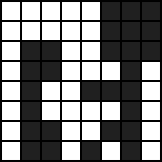
\includegraphics[width=0.25\textwidth]{img/img_telefono.pdf}

    \item Observe que el formato de imagen dado no incluye la paleta de
        colores. ¿Qué problema puede causar esto?

    \item Codifique la siguiente imagen expresando el contenido de su archivo
        en hexadecimal. \label{ej_img_alien}

        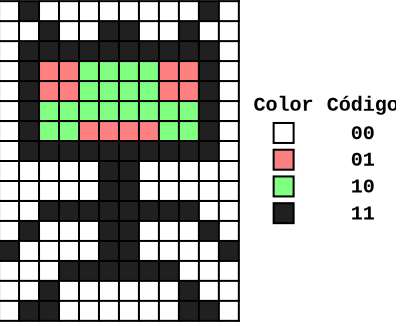
\includegraphics[width=0.5\textwidth]{img/img_alien.pdf}

\end{enumerate}

\section{Compresión}
\label{sec_compresion}

\begin{enumerate}

    \item Dada la siguiente codificación (representada en
        \textbf{hexadecimal}) que corresponde a una imagen:

        \textbf{0C 10 01 40 22 64 7F E7 0E 70 E4 02 4F 27 FE 06 00 60 3F C4 62
        86 10 F0 10 83 0C} \label{ej_img_alien_perdida}

        \begin{enumerate}

            \item Dibuje la imagen resultante considerando una paleta de 2 colores.

            \item ¿Cuántos bits requiere la codificación dada de la imagen? ¿Y
                la del ejercicio \ref{ej_img_alien} de la sección
                ``\textbf{\nameref{sec_imagenes}}''?

            \item ¿Qué técnica de compresión se ha utilizado?

        \end{enumerate}

    \item Considerando la imagen que se muestra abajo, aplique un esquema de
        compresión que agrupa píxeles consecutivos de igual color y los
        reemplaza por una codificación ``\emph{cantidad/color}'', utilizando
        una codificación \textbf{3+1}, con tres bits para la cantidad y un bit
        para el color.

        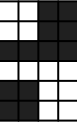
\includegraphics[width=0.25\textwidth]{img/img_comp.pdf}

        \textit{Tenga en cuenta que al calcular la cantidad se debe considerar
        que las filas de la imagen son consecutivas. Es decir, si una fila
        termina con dos pixeles negros y la siguiente comienza con otros dos
        pixeles negros, la codificación debe ser ``4 pixeles negros''}

    \item Si se represente la imagen del ejercicio \ref{ej_img_alien} de la
        sección ``\textbf{\nameref{sec_imagenes}}'' utilizando un esquema de
        compresión ``\emph{cantidad/color}'':

        \begin{enumerate}

            \item ¿De que tipo es la técnica de compresión que utiliza el
                esquema indicado?

            \item ¿Con cuántos bits sería conveniente representar la cantidad?
            ¿y el color?

            \item Mostrar la codificación de la imagen utilizando el esquema
                de compresión indicado.

            \item Comparar la cantidad de bits requeridos para esta
                codificación frente a las de los ejercicios \ref{ej_img_alien} de
                la sección ``\textbf{\nameref{sec_imagenes}}'', y
                \ref{ej_img_alien_perdida} de la sección
                ``\textbf{\nameref{sec_compresion}}''.

        \end{enumerate}

    \item Los formatos de imagen presentados no incluyen toda la información
        necesaria para la decodificación de la imagen.

        \begin{enumerate}

            \item Ademas de la paleta de colores ¿que información agregaría
                para las imágenes comprimidas con y sin perdida? Sugiera una
                nueva cabecera que incluya la información faltante.

            \item  Para poder decodificar una imagen, un programa debe poder
                identificar su tipo ¿Que mecanismo puede utilizar para
                hacerlo? Si es necesario, puede volver a modificar el formato
                de imagen.

        \end{enumerate}

\end{enumerate}

\section{Elaboración de un texto}

\begin{enumerate}

    \item Los informáticos denominamos ``\emph{vuelco de memoria}'' a la
        visualización de los datos contenidos en una región de la memoria. Sea
        el siguiente vuelco de memoria en hexadecimal: \textbf{0x420C701B}.
        ¿Cuáles son sus posibles interpretaciones?

\end{enumerate}

\end{document}
